\documentclass{beamer}
\usepackage{graphicx} % Required for inserting images

\usepackage{amsmath}
\usepackage{amssymb}
\usepackage{amsfonts}
\usepackage{amsthm}
\usepackage{tikz}
\usepackage{tabularx}
\usepackage{multirow}

\usepackage{pgfplots}
\pgfplotsset{compat=1.17}

\title{Convex Optimization Examples}
\author{Jaime Tenorio}
\date{April 2023}

\begin{document}

\maketitle

\begin{frame}
    \frametitle{Convex Optimization}
    A \textit{convex optimization problem} can be stated as

\begin{equation}
    \begin{aligned}
        \text{minimize} \quad& f_0(x) \quad& \\
        \text{subject to} \quad& f_i(x) \leq 0, \quad& i = 1,\ldots,m \\
        \quad& a_i^T x=b_i, \quad& i = 1,\ldots,p, \\
    \end{aligned}
\end{equation}

where the function $f_0(x)$ and the inequality constraints $f_i(x)$ are convex, and the equality constraint must be affine.

The feasible set is convex because it is the intersection of of the domain of the constraints, which are convex. 

\begin{equation}
    D = \bigcap_i^m \textbf{dom} f_i
\end{equation}
\end{frame}

\begin{frame}
    Suppose we have a convex optimization problem where the objective function $f_0$ is differentiable. Let $X$ be the feasible set of the problem. Then $x \in X$ is optimal if and only if:

\begin{equation}
    \nabla f_0(x)^T(y-x) \geq 0 \quad \forall y \in X
\end{equation}

Geometrically, this means that the gradient of the objective function at $x$ points in the direction of the feasible set, in other words, it is a supporting hyperplane to $X$.

\begin{center}
    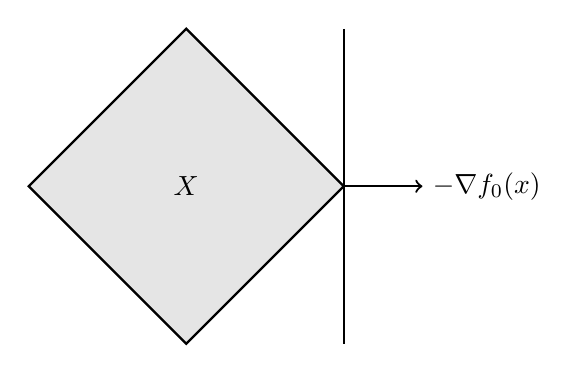
\begin{tikzpicture}[scale=2]
        % Define the convex set X
        \filldraw[fill=gray!20, draw=black] (-1,0) -- (0,1) -- (1,0) -- (0,-1) -- cycle;
        \draw[thick] (-1,0) -- (0,1) -- (1,0) -- (0,-1) -- cycle;

        % Define the tangent line and arrow
        \draw[thick] (1.0,1.0) -- (1.0,-1.0);
        \draw[->,thick] (1.0,0.0) -- (1.5,0.0) node[right]{$-\nabla f_0(x)$};

        % Add the name X to the set
        \node at (0,0) {$X$};
    \end{tikzpicture}
\end{center}

    
\end{frame}

\begin{frame}
    \frametitle{Unconstrained Problems}
    Suppose we have no constraint inequalities $f_i$ and the objective function $f_0$ is differentiable. Then $x \in X$ is optimal if and only if:

\begin{equation}
    \nabla f_0 (x)= 0
\end{equation}
%
Take as an example the \textit{unconstrained quadratic optimization}:

\begin{equation}
    \begin{aligned}
        \text{minimize} & \quad f_0(x) = \frac{1}{2} x^T P x + q^T x + r\\
    \end{aligned}
\end{equation}
%
where $P \in \mathbf{S}_+^n$. The optimality condition gives:

\begin{equation}
    \nabla f_0(x) = P x + q = 0
\end{equation}
\end{frame}

\begin{frame}
    We can visualize this in two dimensions in the following figure:

\begin{center}
    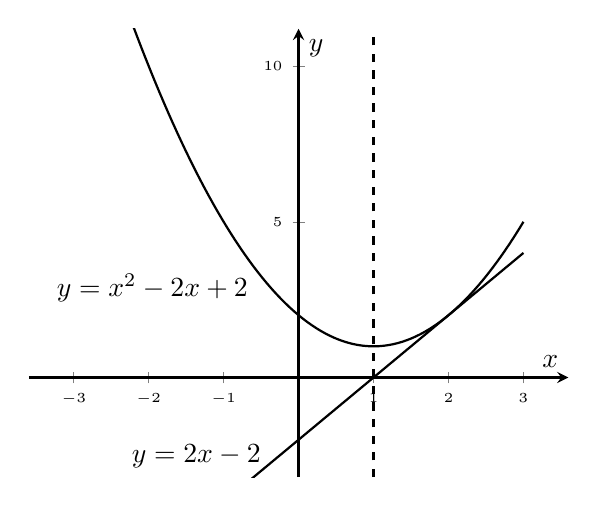
\begin{tikzpicture}[scale=1.0]
        \begin{axis}[
            axis lines=middle,
            xlabel=$x$,
            ylabel=$y$,
            xmin=-3, xmax=3,
            ymin=-2, ymax=10,
            % xtick={-2, -1, 0, 1, 2},
            % ytick={-2, 2, 4, 6, 8, 10},
            ticklabel style={font=\tiny},
            enlargelimits=true,
            thick]
            % Quadratic function
            \addplot[color=black, domain=-3:3, samples=101] {x^2 - 2*x + 2};
            \node[label={-45:{$y=x^2 - 2x + 2$}}] at (axis cs:-3.5,4) {};
            
            % Derivative function
            \addplot[color=black, domain=-3:3, samples=101] {2*x - 2};
            \node[label={-45:{$y=2x-2$}}] at (axis cs:-2.5,-1.5) {};

            \draw[dashed] (1,\pgfkeysvalueof{/pgfplots/ymin}) -- (1,\pgfkeysvalueof{/pgfplots/ymax});
        \end{axis}
    \end{tikzpicture}
\end{center}

\end{frame}

\begin{frame}
    \frametitle{Equality Constraints}
    If we have only equality constraints

\begin{equation}
    \begin{aligned}
        \text{minimize} \quad & f_0(x) \\
        \text{subject to} \quad & Ax=b
    \end{aligned}
\end{equation}
%
the feasible set is affine. The optimality condition for $x \in X$ is

\begin{equation}
    \exists\nu\in\mathbb{R}^p \quad s.t. \quad \nabla f_0(x) + A^T\nu = 0 \quad \text{and} \quad Ax=b
\end{equation}
%
which is the Lagrange multiplier optimality condition, also known as the Karush-Kuhn-Tucker (KKT) condition.

\end{frame}

\begin{frame}
    We can visualize this in two dimensions in the following figure:

\begin{center}
    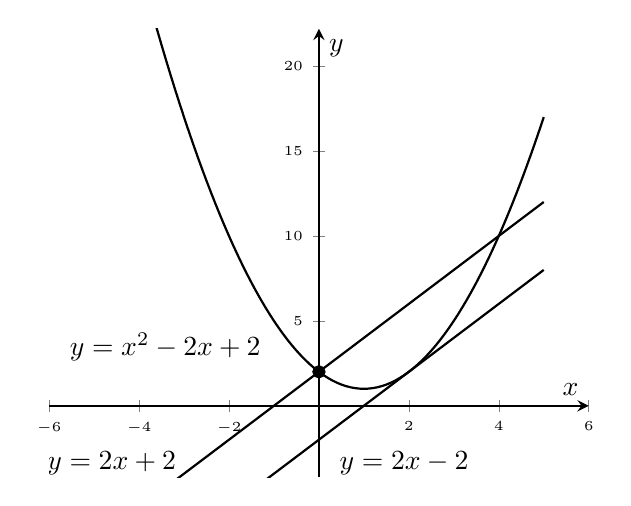
\begin{tikzpicture}[scale=1.0]
        \begin{axis}[
            axis lines=middle,
            xlabel=$x$,
            ylabel=$y$,
            xmin=-5, xmax=5,
            ymin=-2, ymax=20,
            % xtick={-2, -1, 0, 1, 2},
            % ytick={-2, 2, 4, 6, 8, 10},
            ticklabel style={font=\tiny},
            enlargelimits=true,
            thick]

            % Quadratic function
            \addplot[color=black, domain=-5:5, samples=101] {x^2 - 2*x + 2};
            \node[label={-45:{$y=x^2 - 2x + 2$}}] at (axis cs:-6,5.5) {};
            
            % Equality constraint
            \addplot[color=black, domain=-5:5, samples=101] {2*x + 2};
            \node[label={-45:{$y=2x+2$}}] at (axis cs:-6.5,-1.5) {};
            
            % Derivative function
            \addplot[color=black, domain=-5:5, samples=101] {2*x - 2};
            \node[label={-45:{$y=2x-2$}}] at (axis cs:0,-1.5) {};

            \filldraw[black] (0,2) circle (2pt);
        \end{axis}
    \end{tikzpicture}
\end{center}

\end{frame}

\begin{frame}
    \frametitle{Nonnegative Orthant}
    If we consider a problem like

\begin{equation}
    \begin{aligned}
        \text{minimize} \quad & f_0(x) \\
        \text{subject to} \quad & x \succeq 0
    \end{aligned}
\end{equation}
%
where the only constraint is the nonnegativity of $x$. The feasible set is the nonnegative orthant. The optimality condition for $x \succeq 0, x \in X$ is

% \begin{equation}
%     \nabla f_0(x) \succeq 0, \quad x_i(\nabla f_0(x))_i=0, \quad i=1,\ldots,n
% \end{equation}

\begin{equation}
    \begin{cases}
        \nabla f_0(x)_i \geq 0 & x_i=0 \\
        \nabla f_0(x)_i = 0 & x_i>0 \\
    \end{cases}
\end{equation}

\end{frame}

\begin{frame}
    We can visualize this in two dimensions in the following figure:

\begin{center}
    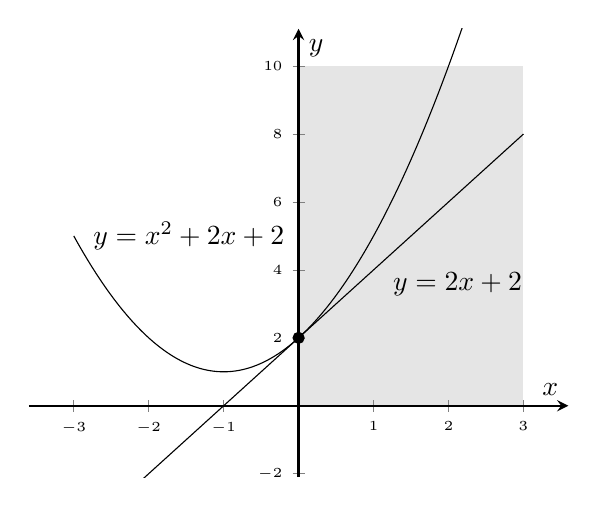
\begin{tikzpicture}[scale=1.0]
        \pgfdeclarelayer{background}
        \pgfdeclarelayer{foreground}
        \pgfsetlayers{background,main,foreground}

        \begin{axis}[
            axis lines=middle,
            xlabel=$x$,
            ylabel=$y$,
            xmin=-3, xmax=3,
            ymin=-1, ymax=10,
            % xtick={-2, -1, 0, 1, 2},
            % ytick={-2, 2, 4, 6, 8, 10},
            ticklabel style={font=\tiny},
            enlargelimits=true,
            thick]

            \begin{pgfonlayer}{background}
                \fill[gray!20] (0,0) rectangle (3,10);
            \end{pgfonlayer}

            % Quadratic function
            \addplot[color=black, domain=-3:3, samples=101] {x^2 + 2*x + 2};
            \node[label={-45:{$y=x^2 + 2x + 2$}}] at (axis cs:-3,6) {};
            
            % Derivative function
            \addplot[color=black, domain=-3:3, samples=101] {2*x + 2};
            \node[label={-45:{$y=2x+2$}}] at (axis cs:1,4.5) {};

            \filldraw[black] (0,2) circle (2pt);
        \end{axis}
    \end{tikzpicture}
\end{center}

\end{frame}

\begin{frame}
    \frametitle{Equivalent Problems}
    \fontsize{10}{10}\selectfont
    We can obtain \textbf{equivalent} convex problems using transformations that preserve convexity.

\begin{center}
    \begin{tabular}{|cc|cc|}
        \hline
        \multicolumn{2}{|c|}{Original} & \multicolumn{2}{|c|}{Equivalent} \\
        \hline
        minimize & $f_0(x)$ & minimize (over $z$) & $f_0(Fz+x_0)$ \\
        subject to& $f_i(x)\leq 0$ & subject to & $f_i(Fz+x_0)$ \\
        & $Ax=b$ & \multicolumn{2}{c|}{$Ax+b \iff x=Fz+x_0$}\\
        \hline
        minimize & $f_0(A_0x+b_0)$ & minimize (over $x,y_i$) & $f_0(y_0)$ \\
        subject to& $f_i(A_ix+b_i)\leq 0$ & subject to & $f_i(y_i)\leq 0$ \\
        & & & $y_i=A_ix+b_i$ \\
        \hline
        minimize & $f_0(x)$ & minimize (over $x,s$) & $f_0(x)$ \\
        subject to& $a_i^Tx\leq b_i$ & subject to & $a_i^Tx+s_i=b_i$ \\
        & & & $s_i\geq0$ \\
        \hline
        minimize & $f_0(x)$ & minimize (over $x,t$) & $t$ \\
        subject to& $f_i(x)\leq0$ & subject to & $f_0(x)-t\leq0$ \\
        & $a_i^Tx=b_i$ & & $f_i(x)\leq0$ \\
        & & & $Ax=b$ \\
        \hline
        minimize & $f_0(x_1,x_2)$ & minimize & $\tilde{f}_0(x_1)$ \\
        subject to& $f_i(x_1)\leq0$ & subject to & $f_i(x_1)\leq0$ \\
        & & \multicolumn{2}{c|}{$\tilde{f}_0(x_1)=\inf_{x_2}{f_0(x_1,x_2)}$}\\
        \hline
    \end{tabular}
\end{center}
%
\end{frame}

\begin{frame}
    %
In the table we can see equivalent problems for the following transformations:

\begin{enumerate}
    \item Eliminating equality constraints 
    \item Introducing equality constraints
    \item Introducing slack variables for linear inequality constraints
    \item Epigraph form of the standard convex problem
    \item Minimizing over some variables
\end{enumerate}
\end{frame}

\begin{frame}
    \frametitle{Neural Network Training}
    Training a neural network can be posed as a convex optimization problem. 

\begin{equation}
    \begin{aligned}
        \text{minimize} \quad& L(y; \hat{y}) \\
        % \text{subject to} \quad& \mathbf{w} \in \mathbb{R}^d
    \end{aligned}
\end{equation}
%
where $L(y; \hat{y})$ is the loss function, $y$ is the ground truth, and $\hat{y}$ is the prediction. The prediction is given by the neural network, which is a function of the weights $W$ and the input $x$. If we consider a network of one layer, the prediction is given by

\begin{equation}
    \hat{y} = \sigma(Wx)
\end{equation}
%
where $\sigma$ is the activation function. For this problem to be convex we need the loss function to be convex. We can consider the following loss functions:
\begin{itemize}
    \item \textbf{Mean squared error (MSE)}: $L(y; \hat{y}) = \frac{1}{2} (y - \hat{y})^2$
    \item \textbf{Cross-entropy loss}: $L(y; \hat{y}) = -y \log(\hat{y}) - (1 - y) \log(1 - \hat{y})$
    \item \textbf{Hinge loss}: $L(y; \hat{y}) = \max(0, 1 - y \hat{y})$
\end{itemize}

\end{frame}

\begin{frame}
    \fontsize{10}{10}\selectfont
    For example, YOLO is a convolutional neural network for object detection. It is trained using the following loss function

\begin{equation}
    \begin{split}
        L=
        &= \lambda_{\text{coord}}
        \sum_{i=0}^{S^2}\sum_{i=0}^{B}\mathbf{1}_{ij}^{\text{obj}}
        \left[(x_i-\hat{x}_i)^2+(y_i-\hat{y}_i)^2\right] \\
        &+ \lambda_{\text{coord}}
        \sum_{i=0}^{S^2}\sum_{i=0}^{B}\mathbf{1}_{ij}^{\text{obj}}
        \left[(\sqrt{w_i}-\sqrt{\hat{w}_i})^2+(\sqrt{h_i}-\sqrt{\hat{h}_i})^2\right] \\
        &+ \sum_{i=0}^{S^2}\sum_{i=0}^{B}\mathbf{1}_{ij}^{\text{obj}}
        \left(C_i-\hat{C}_i\right)^2\\
        &+ \lambda_{\text{noobj}}
        \sum_{i=0}^{S^2}\sum_{i=0}^{B}\mathbf{1}_{ij}^{\text{noobj}}
        \left(C_i-\hat{C}_i\right)^2\\
        &+ \sum_{i=0}^{S^2}\mathbf{1}_{i}^{\text{obj}}\sum_{c\in \text{classes}}
        (p_i(c)-\hat{p}_i(c))^2 \\
    \end{split}
\end{equation}
%
where $\hat{x}, \hat{y}, \hat{w}, \hat{h}, \hat{c}$ are the output from the convolutional neural network. This is a modified mean squared error loss function, which is convex.
\end{frame}

\begin{frame}
    Usually, the optimization of a neural network is not a convex problem.

\begin{figure}[htbp]
\centering
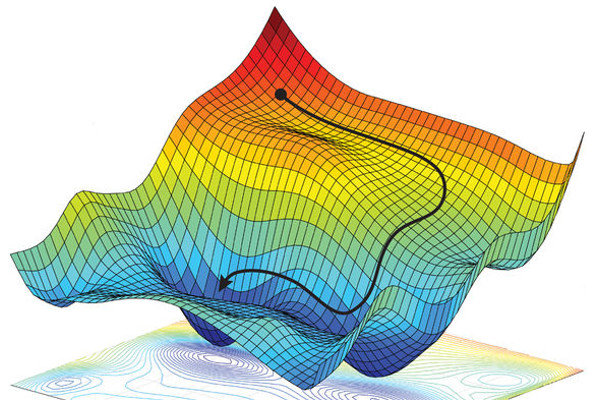
\includegraphics[width=0.8\textwidth]{images/nnopt}
\end{figure}

\end{frame}

\end{document}
